\documentclass{article}
\usepackage{listings}
\usepackage{xcolor}
\usepackage{amsmath}
\usepackage{enumitem}
\usepackage[utf8]{inputenc}
%image ralated package
\usepackage{graphicx}
\usepackage{subcaption}
\usepackage[export]{adjustbox}
\usepackage{wrapfig}
%New colors defined below
\definecolor{codegreen}{rgb}{0,0.6,0}
\definecolor{codegray}{rgb}{0.5,0.5,0.5}
\definecolor{codepurple}{rgb}{0.58,0,0.82}
\definecolor{backcolour}{rgb}{0.95,0.95,0.92}

%Code listing style named "mystyle"
\lstdefinestyle{mystyle}{
  backgroundcolor=\color{backcolour},   commentstyle=\color{codegreen},
  keywordstyle=\color{magenta},
  numberstyle=\tiny\color{codegray},
  stringstyle=\color{codepurple},
  basicstyle=\ttfamily\footnotesize,
  breakatwhitespace=false,         
  breaklines=true,                 
  captionpos=b,                    
  keepspaces=true,                 
  numbers=left,                    
  numbersep=5pt,                  
  showspaces=false,                
  showstringspaces=false,
  showtabs=false,                  
  tabsize=2
}

%"mystyle" code listing set
\lstset{style=mystyle}

\title{0.4, a and b only}
\date{\today}
\author{Yin.Zheng}
\begin{document}

\maketitle

\section{Code examples}

%Importing code from file
\lstinputlisting[language=Python, 
caption=This is O(n) version of my fib matrix
]{/Users/mac/my_ltcd_slt/CS5800/my_fib_matrix.py}

%\clearpage

\lstinputlisting[language=Python, 
caption=This is O(log(n)) version of my fib with matrix
]{/Users/mac/my_ltcd_slt/CS5800/my_fib_v2.py}


\begin{enumerate}[label=(\alph*)]
    \begin{figure}[h]
    \item Q1:Show that two 2 * 2 matrices can multiplied using 4 additions and 8 multiplications.
    But how many matrix multiplications does it take to compute Xn?\\
    
    Answer: In my first version of matrix fib it takes $N-1$ steps to compute $X^n$, 
    Because every time n increases by 1, it is multiplied once more by [0,1,1,1]
    so the time complexity is O(n)\\
     \\
        
        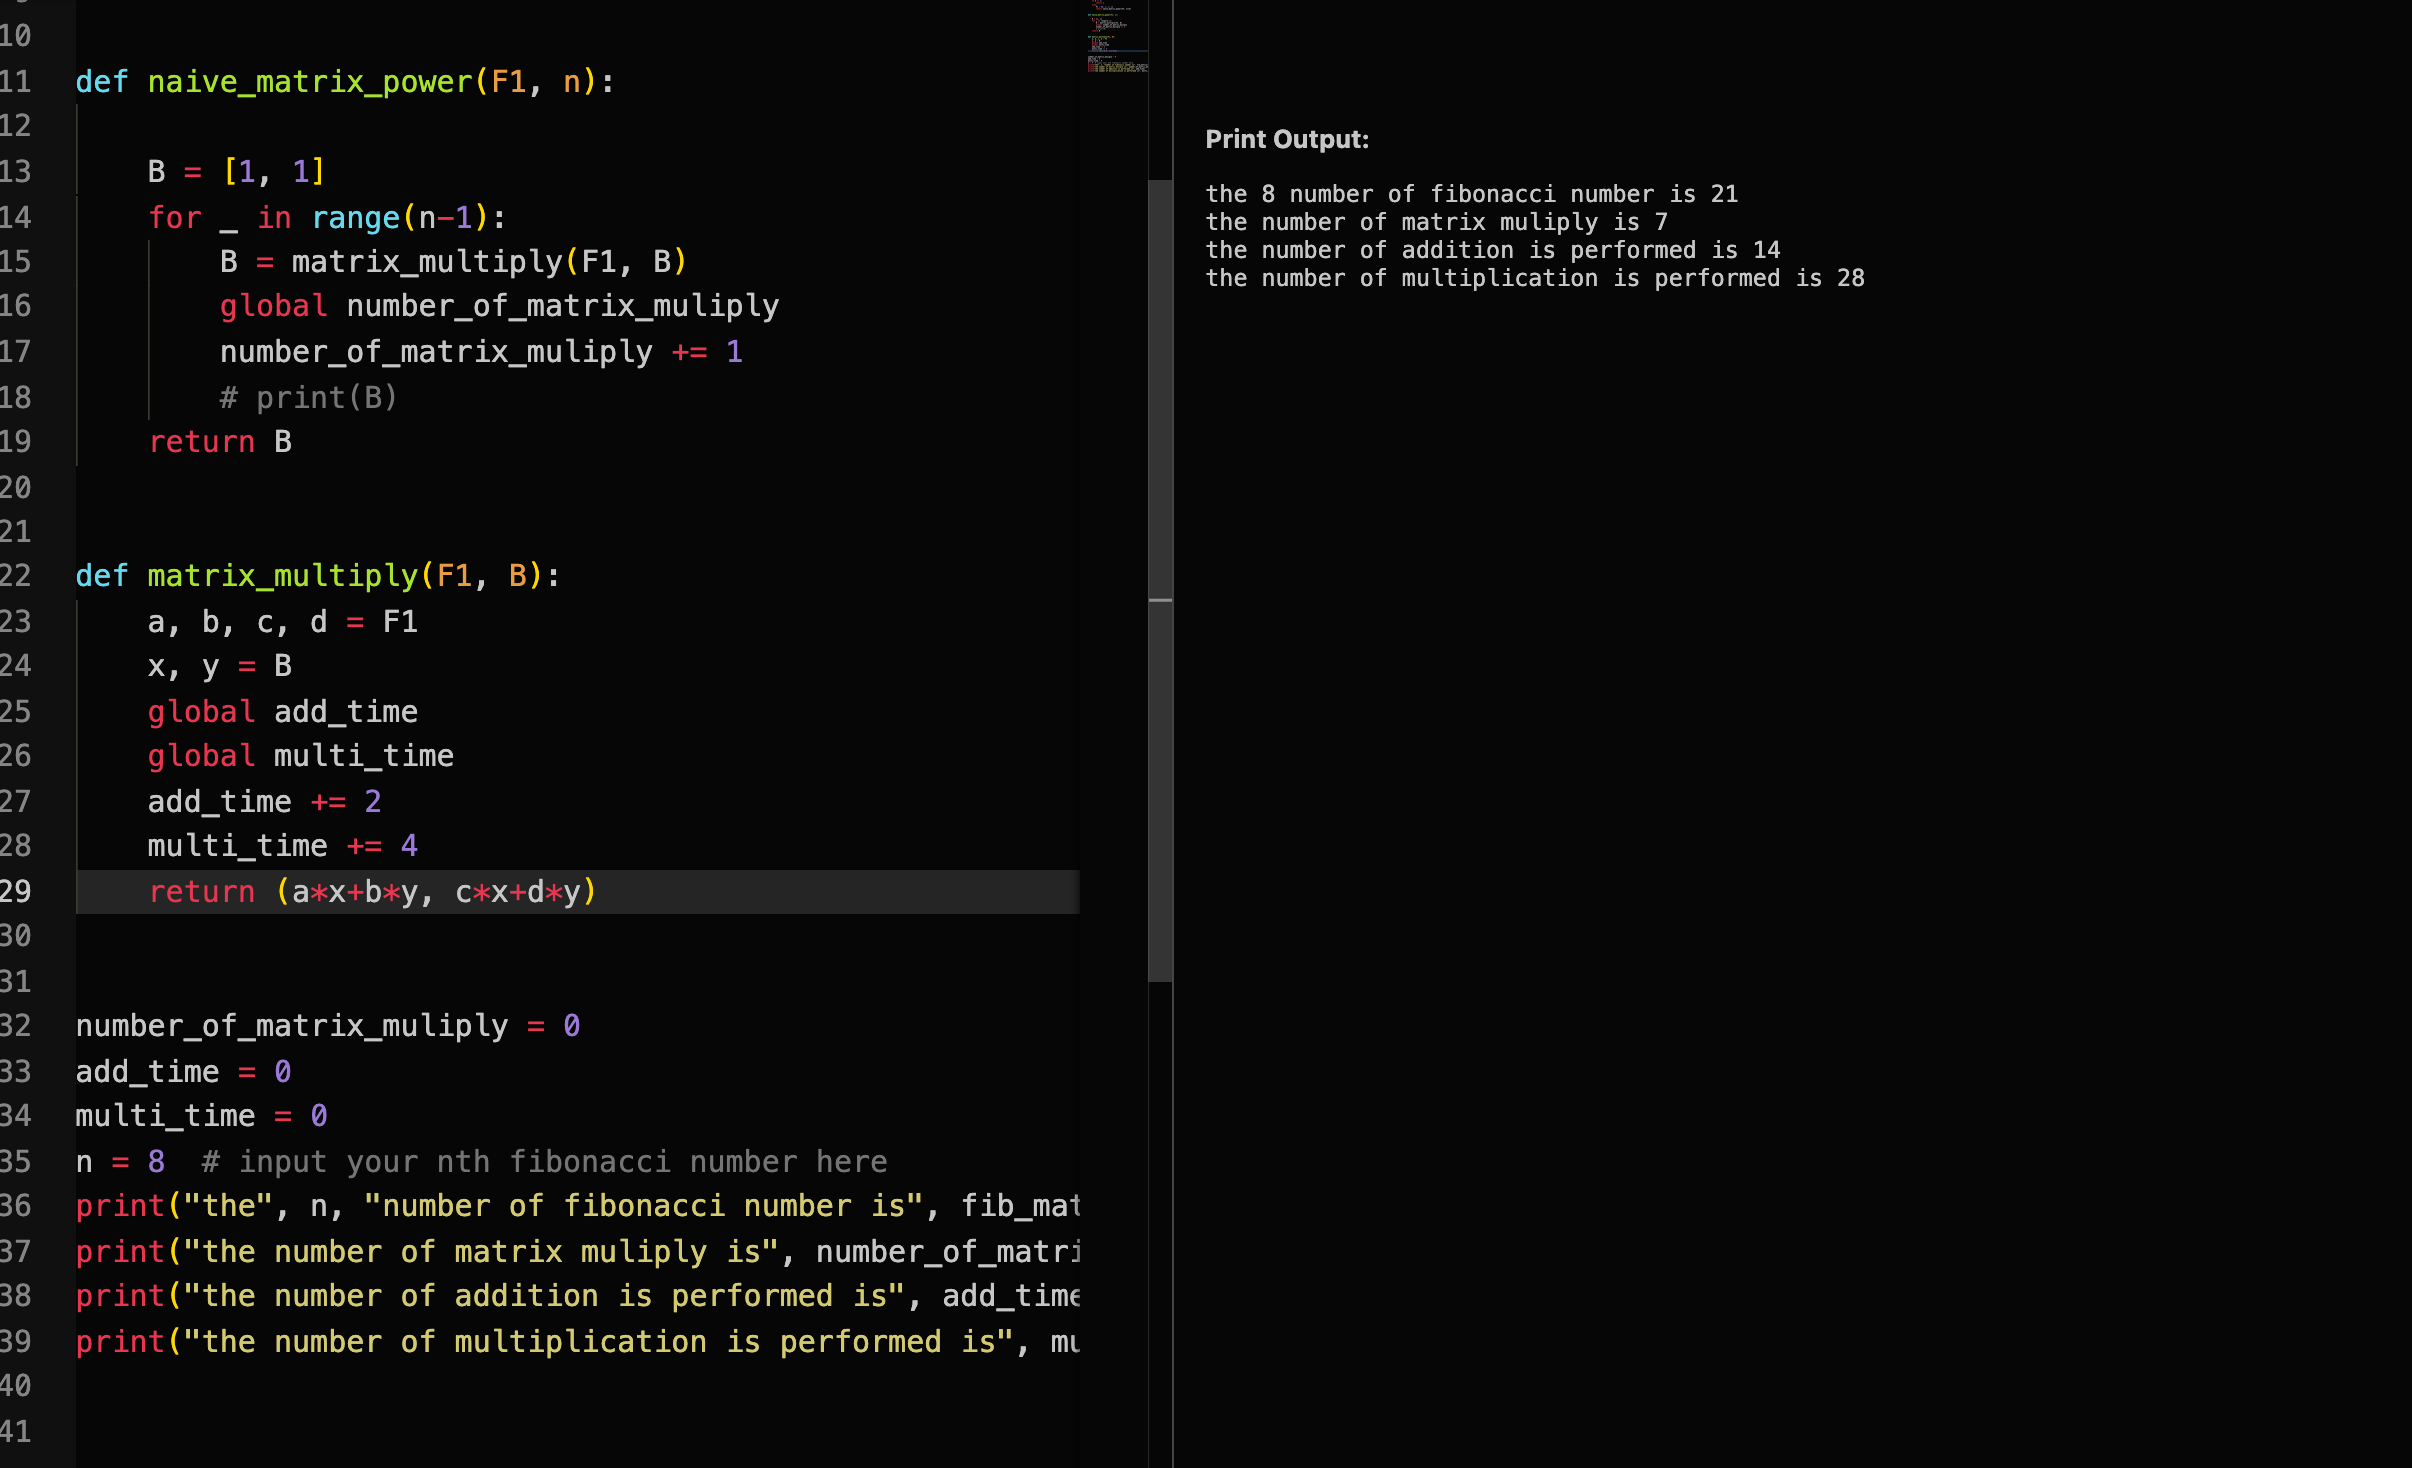
\includegraphics[width=1.5\textwidth, inner]{ss for q1.png}
        \caption{Screen shot for Q1}
        \label{fig:figure1}
        \end{figure}
    

    \begin{figure}[h]
    \item Q2:Show that O(logn) matrix multiplications suffice for computing Xn. (Hint:Think about computing X8.)\\
    Answer:In my second version of matrix Fib, it takes it takes $log(n)$ steps to compute $X^n$
    Because in this version matrix Multiplication grows exponentially\\
    \noindent For example when n=8, we are calculating the 8th fib number. This is what happens in this loop:
    \begin{lstlisting}[language=Python, caption=loop code]
        while i <= n:
            # repeated square B until n = 2^q > m
            B = matrix_multiply_f2(B, B)
            global global_N
            global_N += 1
            i = i*2
        \end{lstlisting}
    \begin{itemize}
        \item When i=2 B became $B^2$
        \item when i=4 $B^2$ became $B^4$
        \item when i=8 $B^4$ became $B^8$
        \item when i=16 jump out of the loop
    \end{itemize}
As you can see the matrix multiply function execute 3 times, $3=log(8)$,so $O(logn)$ matrix multiplications suffice for computing $X^n$\\

    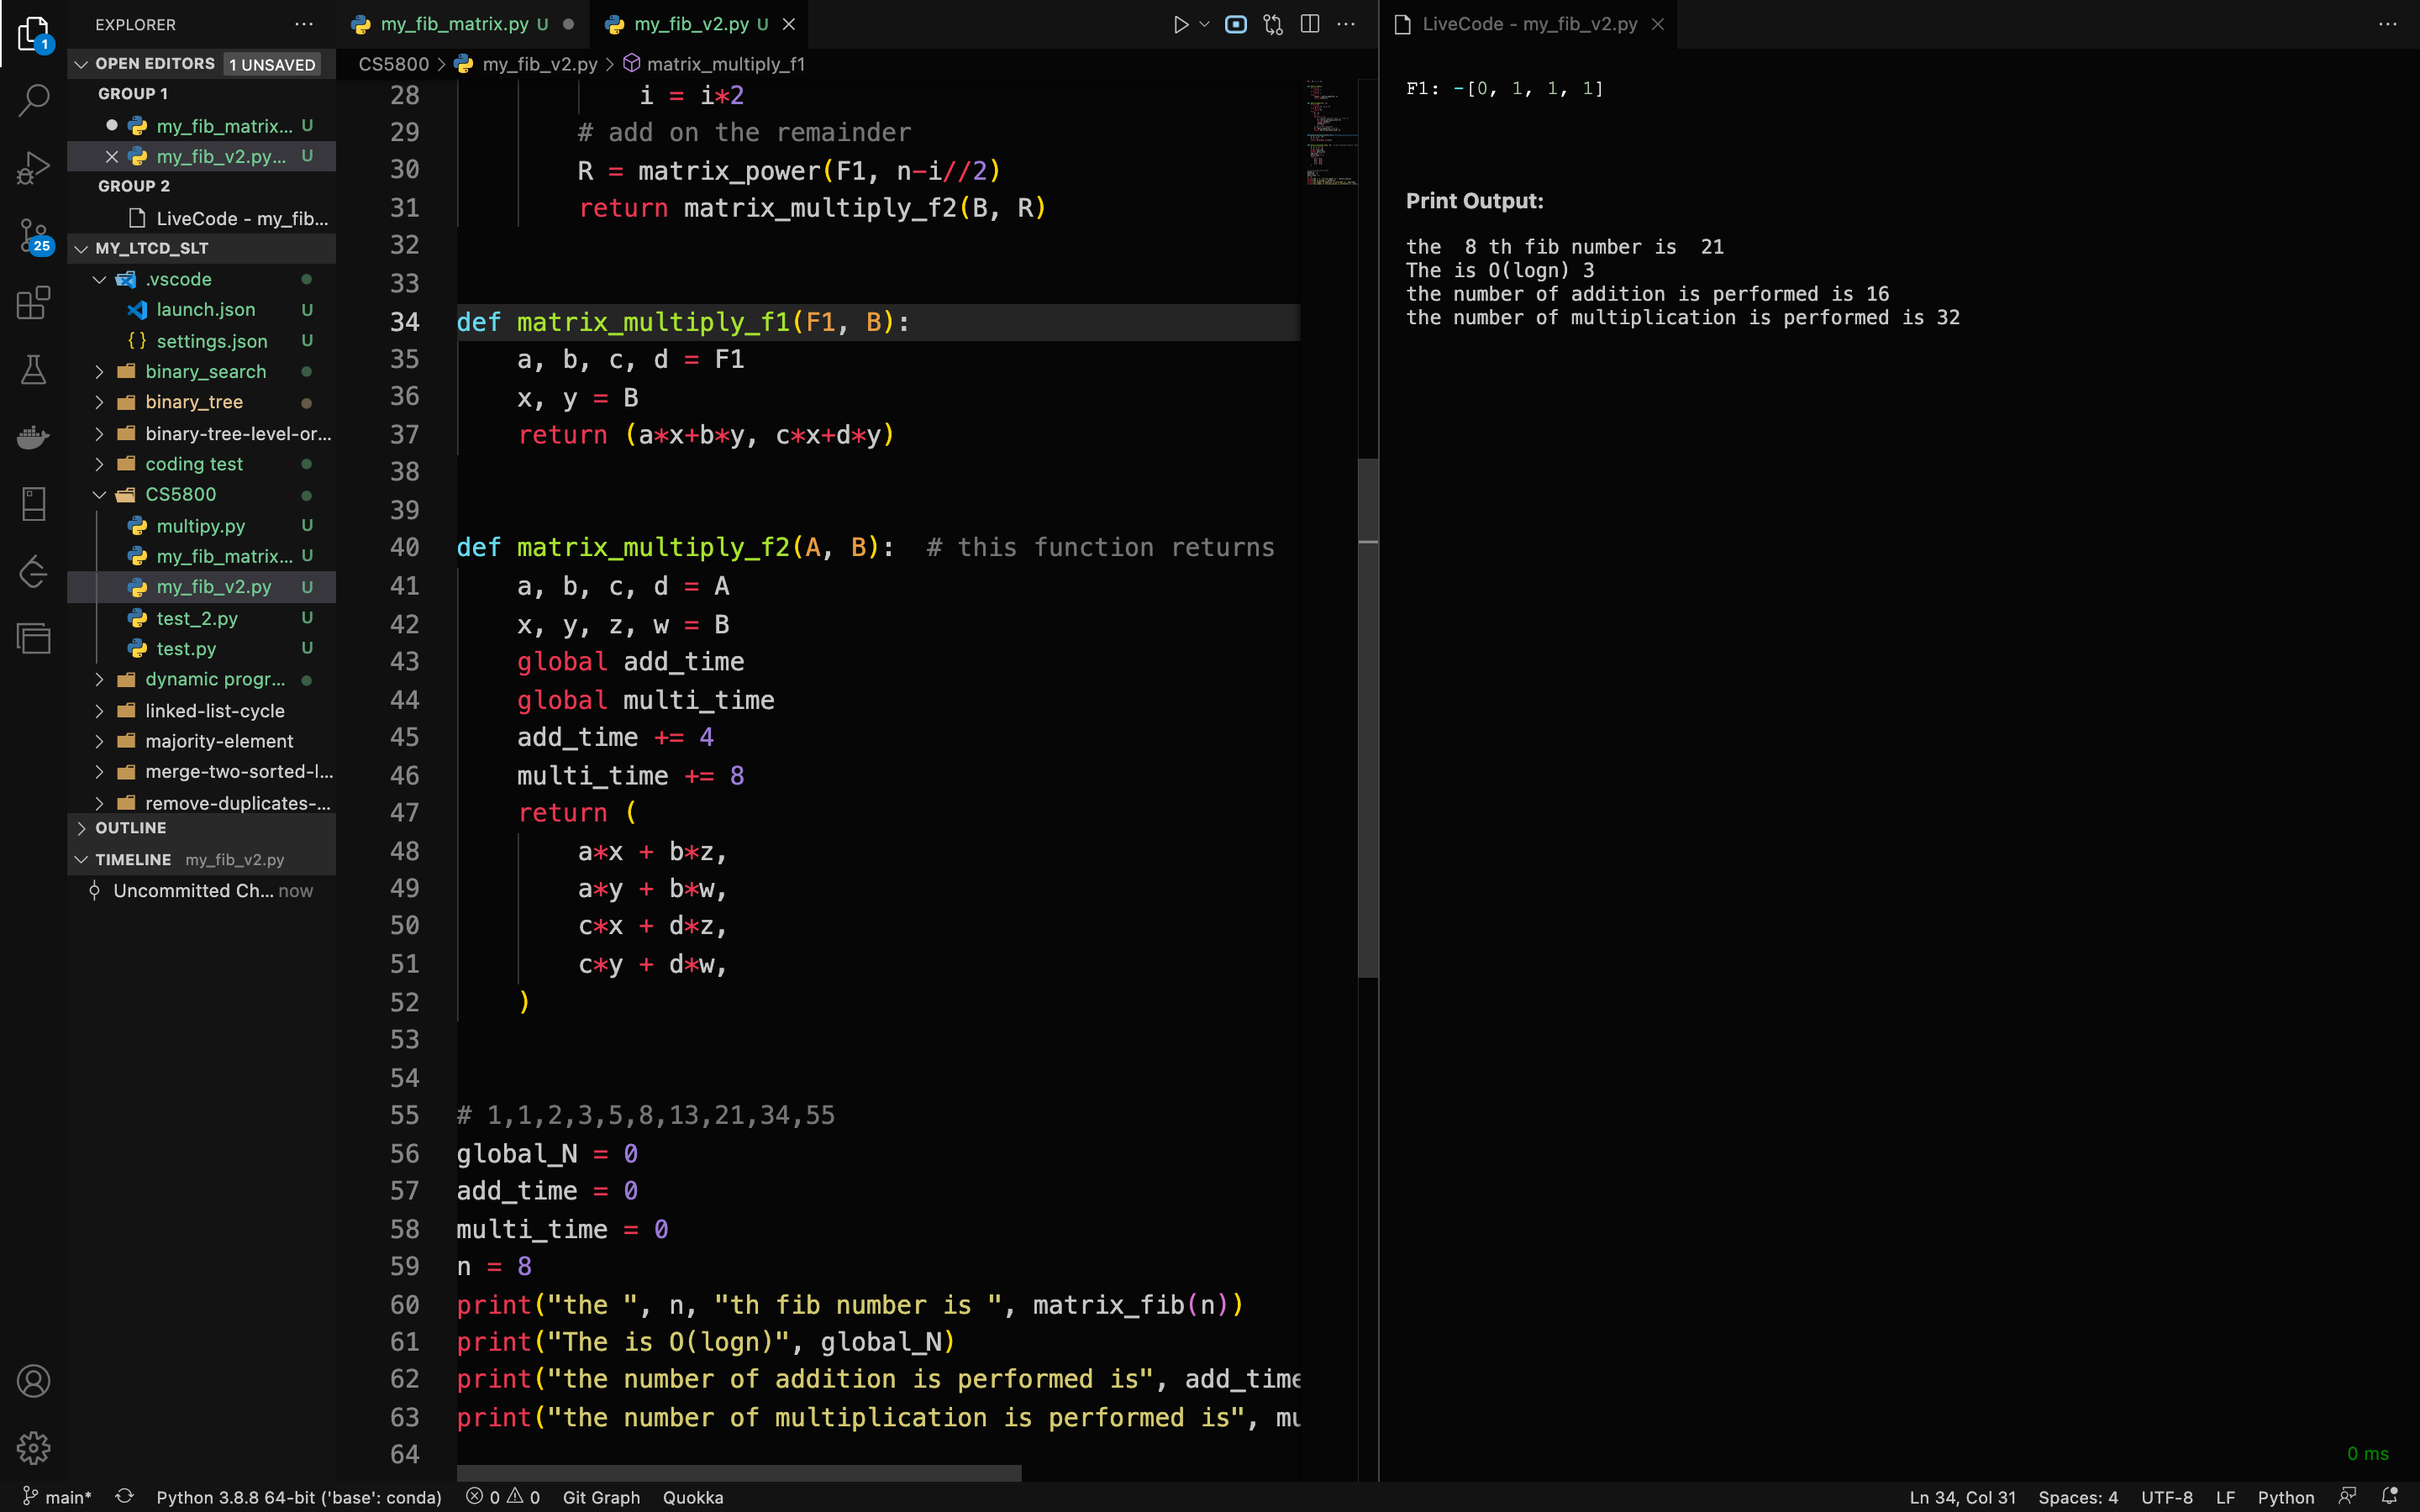
\includegraphics[width=1.5\textwidth, inner]{ss fdr q2}
    \caption{Screen shot for Q2}
    \label{fig:figure2}
    \end{figure}
\end{enumerate}

\end{document}


\end{document}